% Options for packages loaded elsewhere
\PassOptionsToPackage{unicode}{hyperref}
\PassOptionsToPackage{hyphens}{url}
%
\documentclass[
]{article}
\usepackage{amsmath,amssymb}
\usepackage{lmodern}
\usepackage{ifxetex,ifluatex}
\ifnum 0\ifxetex 1\fi\ifluatex 1\fi=0 % if pdftex
  \usepackage[T1]{fontenc}
  \usepackage[utf8]{inputenc}
  \usepackage{textcomp} % provide euro and other symbols
\else % if luatex or xetex
  \usepackage{unicode-math}
  \defaultfontfeatures{Scale=MatchLowercase}
  \defaultfontfeatures[\rmfamily]{Ligatures=TeX,Scale=1}
\fi
% Use upquote if available, for straight quotes in verbatim environments
\IfFileExists{upquote.sty}{\usepackage{upquote}}{}
\IfFileExists{microtype.sty}{% use microtype if available
  \usepackage[]{microtype}
  \UseMicrotypeSet[protrusion]{basicmath} % disable protrusion for tt fonts
}{}
\makeatletter
\@ifundefined{KOMAClassName}{% if non-KOMA class
  \IfFileExists{parskip.sty}{%
    \usepackage{parskip}
  }{% else
    \setlength{\parindent}{0pt}
    \setlength{\parskip}{6pt plus 2pt minus 1pt}}
}{% if KOMA class
  \KOMAoptions{parskip=half}}
\makeatother
\usepackage{xcolor}
\IfFileExists{xurl.sty}{\usepackage{xurl}}{} % add URL line breaks if available
\IfFileExists{bookmark.sty}{\usepackage{bookmark}}{\usepackage{hyperref}}
\hypersetup{
  pdftitle={GDE behavior exploiration},
  pdfauthor={Connor French},
  hidelinks,
  pdfcreator={LaTeX via pandoc}}
\urlstyle{same} % disable monospaced font for URLs
\usepackage[margin=1in]{geometry}
\usepackage{color}
\usepackage{fancyvrb}
\newcommand{\VerbBar}{|}
\newcommand{\VERB}{\Verb[commandchars=\\\{\}]}
\DefineVerbatimEnvironment{Highlighting}{Verbatim}{commandchars=\\\{\}}
% Add ',fontsize=\small' for more characters per line
\usepackage{framed}
\definecolor{shadecolor}{RGB}{248,248,248}
\newenvironment{Shaded}{\begin{snugshade}}{\end{snugshade}}
\newcommand{\AlertTok}[1]{\textcolor[rgb]{0.94,0.16,0.16}{#1}}
\newcommand{\AnnotationTok}[1]{\textcolor[rgb]{0.56,0.35,0.01}{\textbf{\textit{#1}}}}
\newcommand{\AttributeTok}[1]{\textcolor[rgb]{0.77,0.63,0.00}{#1}}
\newcommand{\BaseNTok}[1]{\textcolor[rgb]{0.00,0.00,0.81}{#1}}
\newcommand{\BuiltInTok}[1]{#1}
\newcommand{\CharTok}[1]{\textcolor[rgb]{0.31,0.60,0.02}{#1}}
\newcommand{\CommentTok}[1]{\textcolor[rgb]{0.56,0.35,0.01}{\textit{#1}}}
\newcommand{\CommentVarTok}[1]{\textcolor[rgb]{0.56,0.35,0.01}{\textbf{\textit{#1}}}}
\newcommand{\ConstantTok}[1]{\textcolor[rgb]{0.00,0.00,0.00}{#1}}
\newcommand{\ControlFlowTok}[1]{\textcolor[rgb]{0.13,0.29,0.53}{\textbf{#1}}}
\newcommand{\DataTypeTok}[1]{\textcolor[rgb]{0.13,0.29,0.53}{#1}}
\newcommand{\DecValTok}[1]{\textcolor[rgb]{0.00,0.00,0.81}{#1}}
\newcommand{\DocumentationTok}[1]{\textcolor[rgb]{0.56,0.35,0.01}{\textbf{\textit{#1}}}}
\newcommand{\ErrorTok}[1]{\textcolor[rgb]{0.64,0.00,0.00}{\textbf{#1}}}
\newcommand{\ExtensionTok}[1]{#1}
\newcommand{\FloatTok}[1]{\textcolor[rgb]{0.00,0.00,0.81}{#1}}
\newcommand{\FunctionTok}[1]{\textcolor[rgb]{0.00,0.00,0.00}{#1}}
\newcommand{\ImportTok}[1]{#1}
\newcommand{\InformationTok}[1]{\textcolor[rgb]{0.56,0.35,0.01}{\textbf{\textit{#1}}}}
\newcommand{\KeywordTok}[1]{\textcolor[rgb]{0.13,0.29,0.53}{\textbf{#1}}}
\newcommand{\NormalTok}[1]{#1}
\newcommand{\OperatorTok}[1]{\textcolor[rgb]{0.81,0.36,0.00}{\textbf{#1}}}
\newcommand{\OtherTok}[1]{\textcolor[rgb]{0.56,0.35,0.01}{#1}}
\newcommand{\PreprocessorTok}[1]{\textcolor[rgb]{0.56,0.35,0.01}{\textit{#1}}}
\newcommand{\RegionMarkerTok}[1]{#1}
\newcommand{\SpecialCharTok}[1]{\textcolor[rgb]{0.00,0.00,0.00}{#1}}
\newcommand{\SpecialStringTok}[1]{\textcolor[rgb]{0.31,0.60,0.02}{#1}}
\newcommand{\StringTok}[1]{\textcolor[rgb]{0.31,0.60,0.02}{#1}}
\newcommand{\VariableTok}[1]{\textcolor[rgb]{0.00,0.00,0.00}{#1}}
\newcommand{\VerbatimStringTok}[1]{\textcolor[rgb]{0.31,0.60,0.02}{#1}}
\newcommand{\WarningTok}[1]{\textcolor[rgb]{0.56,0.35,0.01}{\textbf{\textit{#1}}}}
\usepackage{graphicx}
\makeatletter
\def\maxwidth{\ifdim\Gin@nat@width>\linewidth\linewidth\else\Gin@nat@width\fi}
\def\maxheight{\ifdim\Gin@nat@height>\textheight\textheight\else\Gin@nat@height\fi}
\makeatother
% Scale images if necessary, so that they will not overflow the page
% margins by default, and it is still possible to overwrite the defaults
% using explicit options in \includegraphics[width, height, ...]{}
\setkeys{Gin}{width=\maxwidth,height=\maxheight,keepaspectratio}
% Set default figure placement to htbp
\makeatletter
\def\fps@figure{htbp}
\makeatother
\setlength{\emergencystretch}{3em} % prevent overfull lines
\providecommand{\tightlist}{%
  \setlength{\itemsep}{0pt}\setlength{\parskip}{0pt}}
\setcounter{secnumdepth}{-\maxdimen} % remove section numbering
\ifluatex
  \usepackage{selnolig}  % disable illegal ligatures
\fi

\title{GDE behavior exploiration}
\author{Connor French}
\date{}

\begin{document}
\maketitle

Goals:

\begin{itemize}
\tightlist
\item
  figure out behavior of GDE when correcting for sampling. Does it vary
  across sample sizes?

  \begin{itemize}
  \tightlist
  \item
    short answer- lower samples mean more variation in GDE calculation
  \item
    makes sense, given higher sample size for simulated distribution =
    more precise estimate of its shape
  \end{itemize}
\item
  Gain intuition for processes leading to different values of GDE\\
\item
  Have a coherent explanation for paper
\end{itemize}

\hypertarget{goal-1--sample-size}{%
\section{Goal 1- sample size}\label{goal-1--sample-size}}

Goal 1 strategy:

\begin{itemize}
\tightlist
\item
  Generate distributions of genetic diversity with different sample
  sizes and shapes
\item
  calculate corrected Hill 1 for each, and see if it varies across
  sample sizes
\end{itemize}

\begin{Shaded}
\begin{Highlighting}[]
\FunctionTok{library}\NormalTok{(tidyverse)}
\end{Highlighting}
\end{Shaded}

\begin{verbatim}
## -- Attaching packages --------------------------------------- tidyverse 1.3.1 --
\end{verbatim}

\begin{verbatim}
## v ggplot2 3.3.3     v purrr   0.3.4
## v tibble  3.1.2     v dplyr   1.0.6
## v tidyr   1.1.3     v stringr 1.4.0
## v readr   1.4.0     v forcats 0.5.1
\end{verbatim}

\begin{verbatim}
## -- Conflicts ------------------------------------------ tidyverse_conflicts() --
## x dplyr::filter() masks stats::filter()
## x dplyr::lag()    masks stats::lag()
\end{verbatim}

\begin{Shaded}
\begin{Highlighting}[]
\FunctionTok{library}\NormalTok{(here)}
\end{Highlighting}
\end{Shaded}

\begin{verbatim}
## here() starts at /Users/connorfrench/Dropbox/Old_Mac/School_Stuff/CUNY/BigAss-bird-phylogeography/BigAss-phylogeography
\end{verbatim}

\begin{Shaded}
\begin{Highlighting}[]
\FunctionTok{source}\NormalTok{(}\FunctionTok{here}\NormalTok{(}\StringTok{"R"}\NormalTok{, }\StringTok{"helper\_functions.R"}\NormalTok{))}
\end{Highlighting}
\end{Shaded}

vector of sample sizes to work with. from 50 to 1000 ``species''.
sorting from lowest to highest sample sizes to make interpretation easy.

\begin{Shaded}
\begin{Highlighting}[]
\FunctionTok{set.seed}\NormalTok{(}\DecValTok{400}\NormalTok{)}
\NormalTok{sample\_sizes }\OtherTok{\textless{}{-}} \FunctionTok{runif}\NormalTok{(}\DecValTok{200}\NormalTok{, }\AttributeTok{min =} \DecValTok{50}\NormalTok{, }\AttributeTok{max =} \DecValTok{1000}\NormalTok{) }\SpecialCharTok{\%\textgreater{}\%} 
  \FunctionTok{round}\NormalTok{() }\SpecialCharTok{\%\textgreater{}\%} 
  \FunctionTok{sort}\NormalTok{()}
\end{Highlighting}
\end{Shaded}

\hypertarget{low-evenness}{%
\subsection{Low evenness}\label{low-evenness}}

generate beta distributions for each sample size

\begin{Shaded}
\begin{Highlighting}[]
\FunctionTok{set.seed}\NormalTok{(}\DecValTok{550}\NormalTok{)}
\NormalTok{low\_even }\OtherTok{\textless{}{-}} \FunctionTok{map}\NormalTok{(sample\_sizes, }\SpecialCharTok{\textasciitilde{}}\FunctionTok{rbeta}\NormalTok{(.x, }\FloatTok{0.2}\NormalTok{, }\DecValTok{3}\NormalTok{)) }
\end{Highlighting}
\end{Shaded}

An example distribution for low hill number

\begin{Shaded}
\begin{Highlighting}[]
\FunctionTok{hist}\NormalTok{(low\_even[[}\DecValTok{150}\NormalTok{]])}
\end{Highlighting}
\end{Shaded}

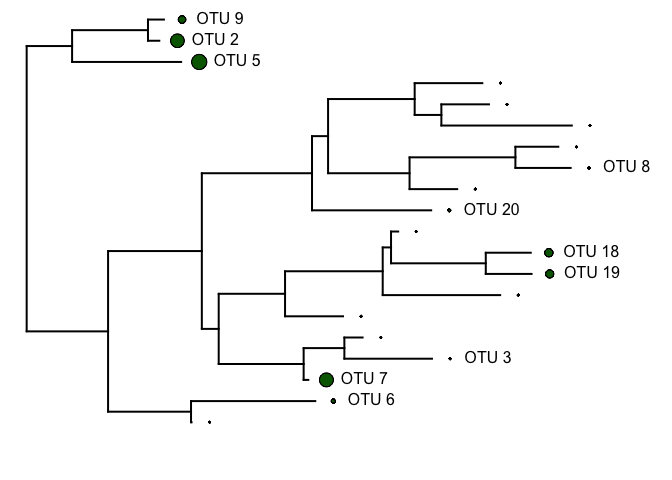
\includegraphics{gde_behavior_exploration_files/figure-latex/unnamed-chunk-3-1.pdf}

sorted bar plot for low evenness

\begin{Shaded}
\begin{Highlighting}[]
\FunctionTok{barplot}\NormalTok{(}\FunctionTok{sort}\NormalTok{(low\_even[[}\DecValTok{150}\NormalTok{]], }\AttributeTok{decreasing =} \ConstantTok{TRUE}\NormalTok{))}
\end{Highlighting}
\end{Shaded}

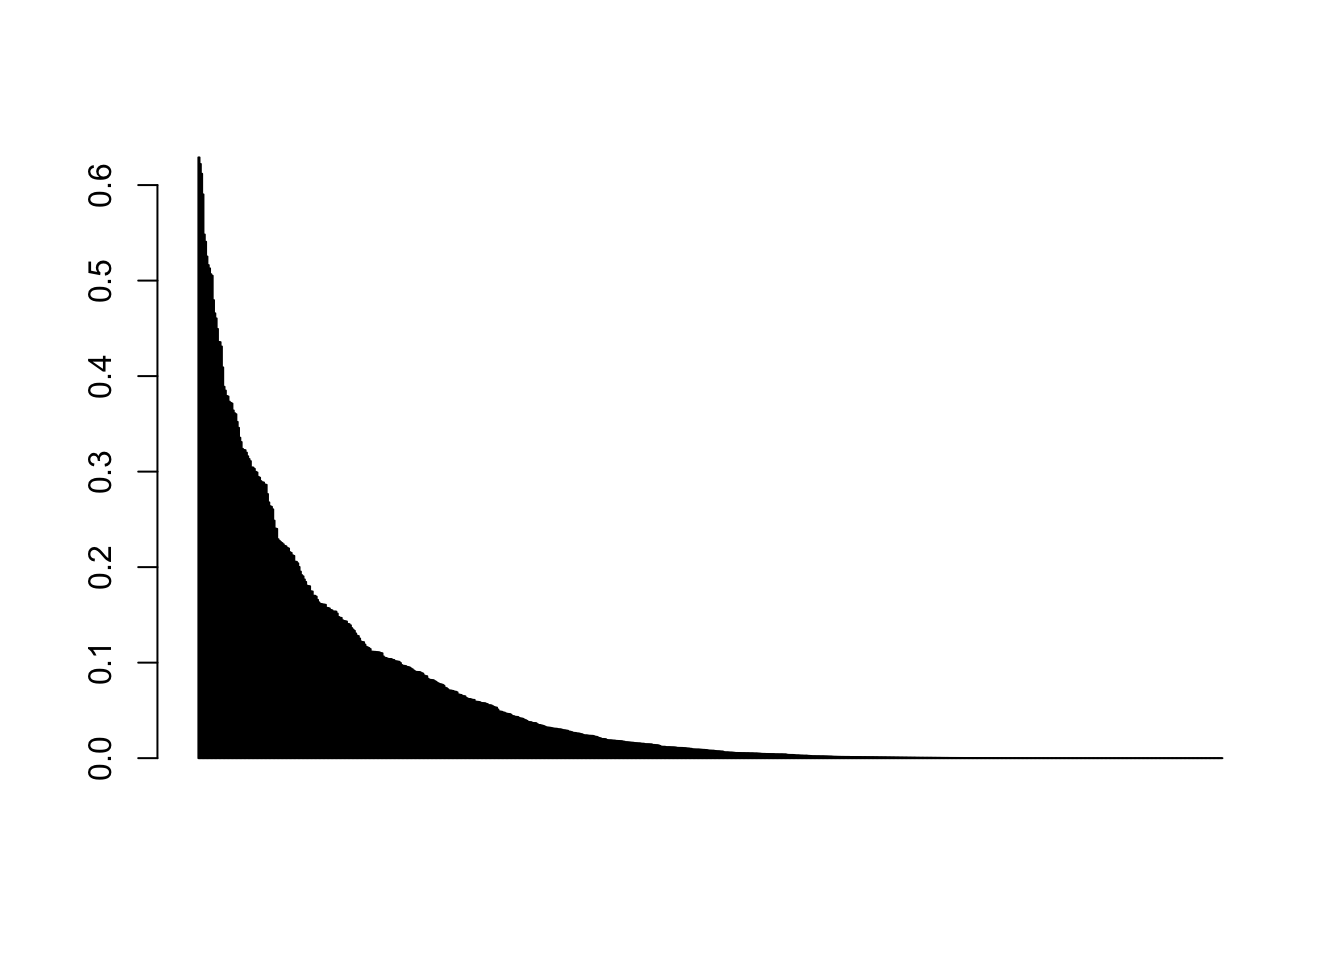
\includegraphics{gde_behavior_exploration_files/figure-latex/unnamed-chunk-4-1.pdf}

calculate hill numbers for each sample size

\begin{Shaded}
\begin{Highlighting}[]
\NormalTok{low\_even\_hill }\OtherTok{\textless{}{-}} \FunctionTok{map}\NormalTok{(low\_even, hill\_calc)}
\end{Highlighting}
\end{Shaded}

hill numbers are concentrated \textasciitilde0.31

\begin{Shaded}
\begin{Highlighting}[]
\FunctionTok{hist}\NormalTok{(}\FunctionTok{unlist}\NormalTok{(low\_even\_hill))}
\end{Highlighting}
\end{Shaded}

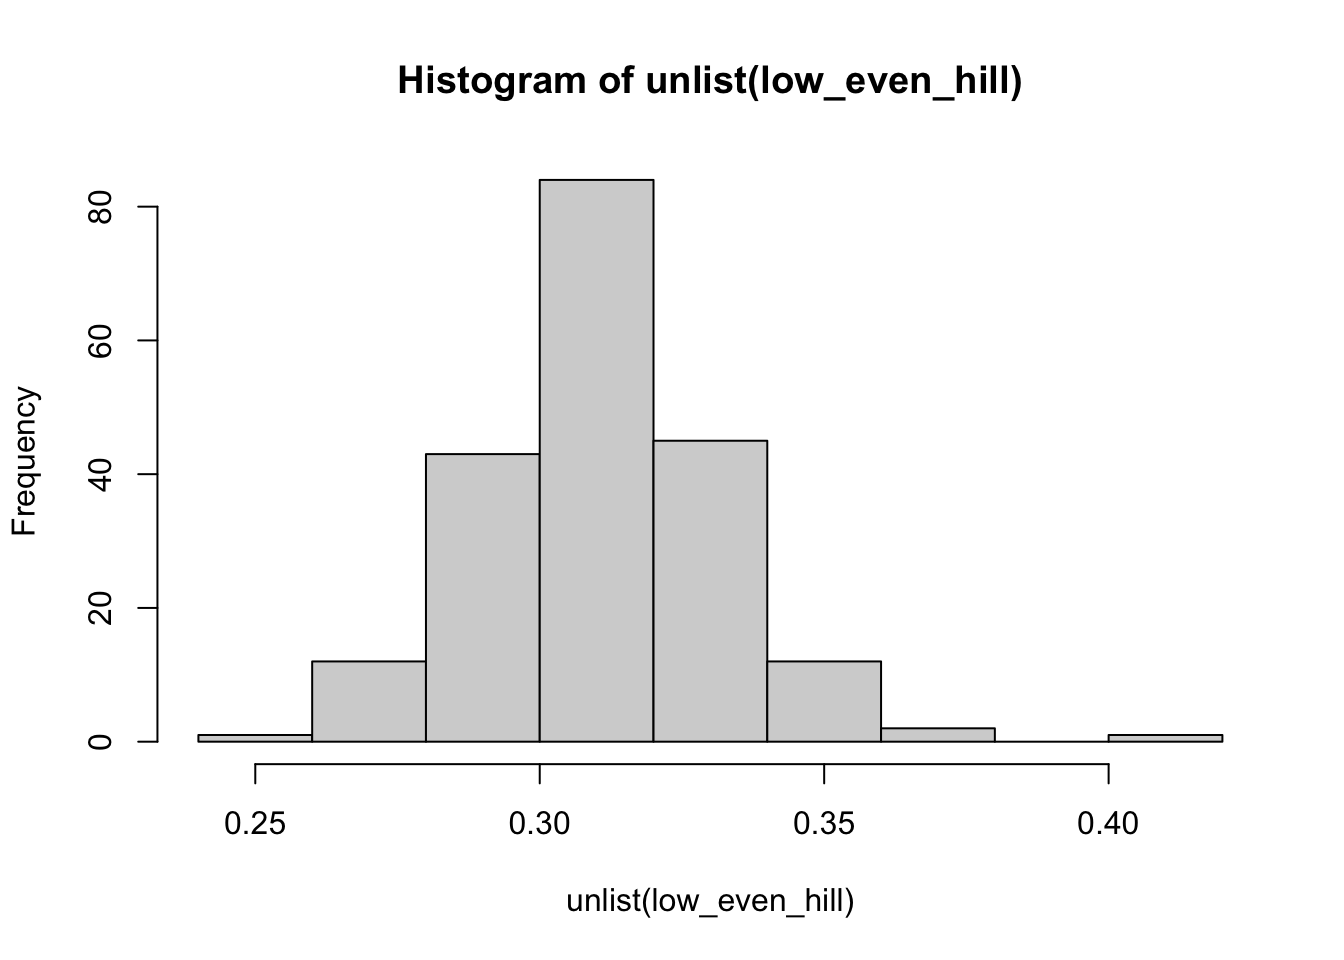
\includegraphics{gde_behavior_exploration_files/figure-latex/unnamed-chunk-6-1.pdf}

since the sample size vector is sorted, lower indices are lower sample
sizes.\\
looks like there is more variation at lower sample sizes.

\begin{Shaded}
\begin{Highlighting}[]
\FunctionTok{plot}\NormalTok{(}\FunctionTok{unlist}\NormalTok{(low\_even\_hill))}
\end{Highlighting}
\end{Shaded}

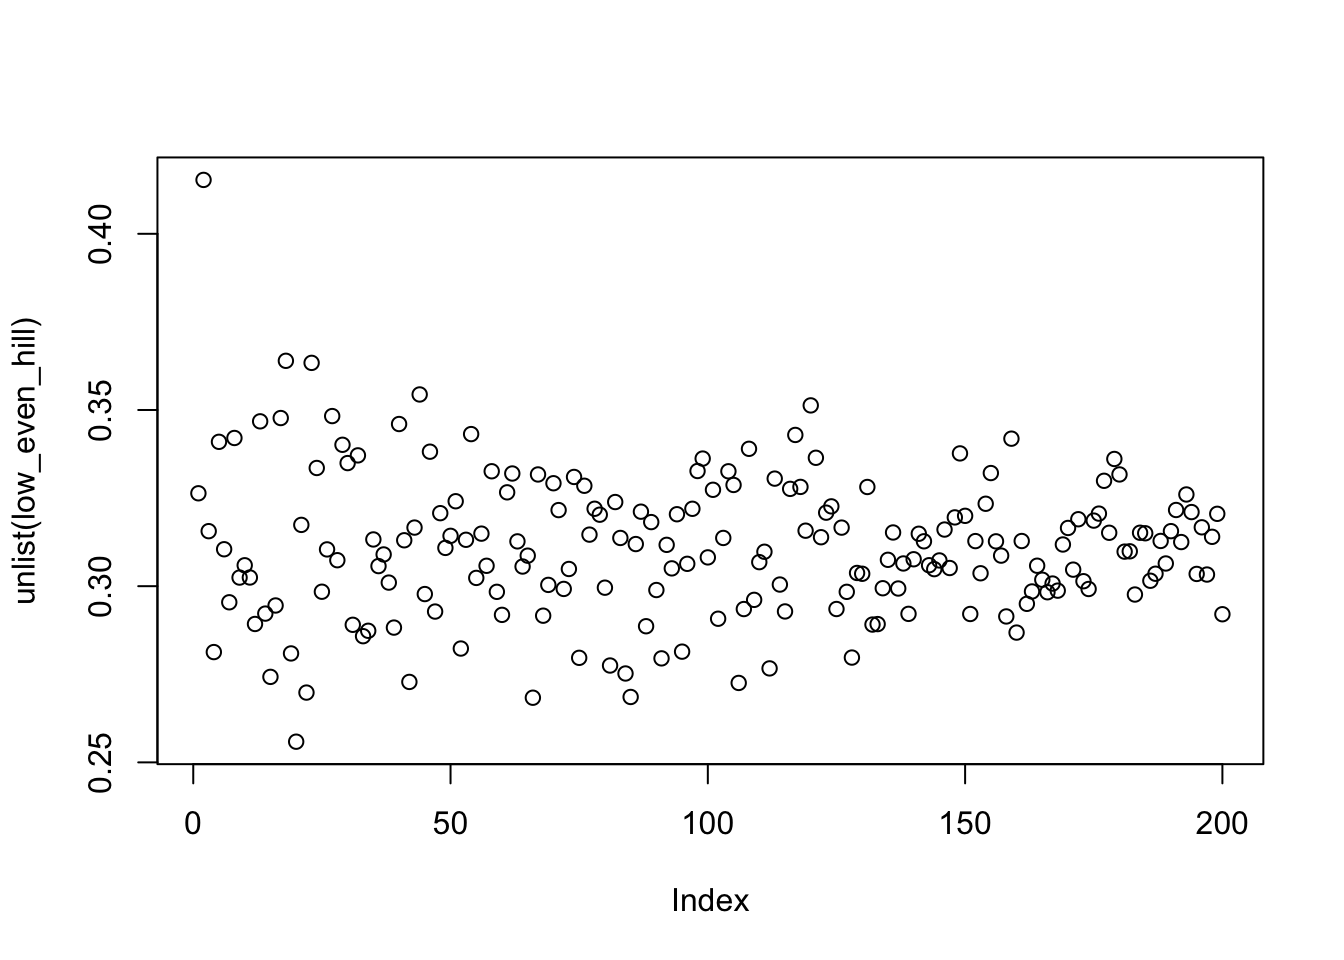
\includegraphics{gde_behavior_exploration_files/figure-latex/unnamed-chunk-7-1.pdf}

\hypertarget{high-evenness}{%
\subsection{High evenness}\label{high-evenness}}

Go through the same steps as low evenness\\
We also see more variaion at low sample sizes vs.~higher sample sizes.
Makes sense.

\begin{Shaded}
\begin{Highlighting}[]
\CommentTok{\# generate beta distributions for each sample size }
\NormalTok{hi\_even }\OtherTok{\textless{}{-}} \FunctionTok{map}\NormalTok{(sample\_sizes, }\SpecialCharTok{\textasciitilde{}}\FunctionTok{rbeta}\NormalTok{(.x, }\DecValTok{3}\NormalTok{, }\DecValTok{3}\NormalTok{)) }

\CommentTok{\# calculate hill numbers for each sample size}
\NormalTok{hi\_even\_hill }\OtherTok{\textless{}{-}} \FunctionTok{map}\NormalTok{(hi\_even, hill\_calc)}
\end{Highlighting}
\end{Shaded}

example distribution for high hill number

\begin{Shaded}
\begin{Highlighting}[]
\FunctionTok{hist}\NormalTok{(hi\_even[[}\DecValTok{150}\NormalTok{]])}
\end{Highlighting}
\end{Shaded}

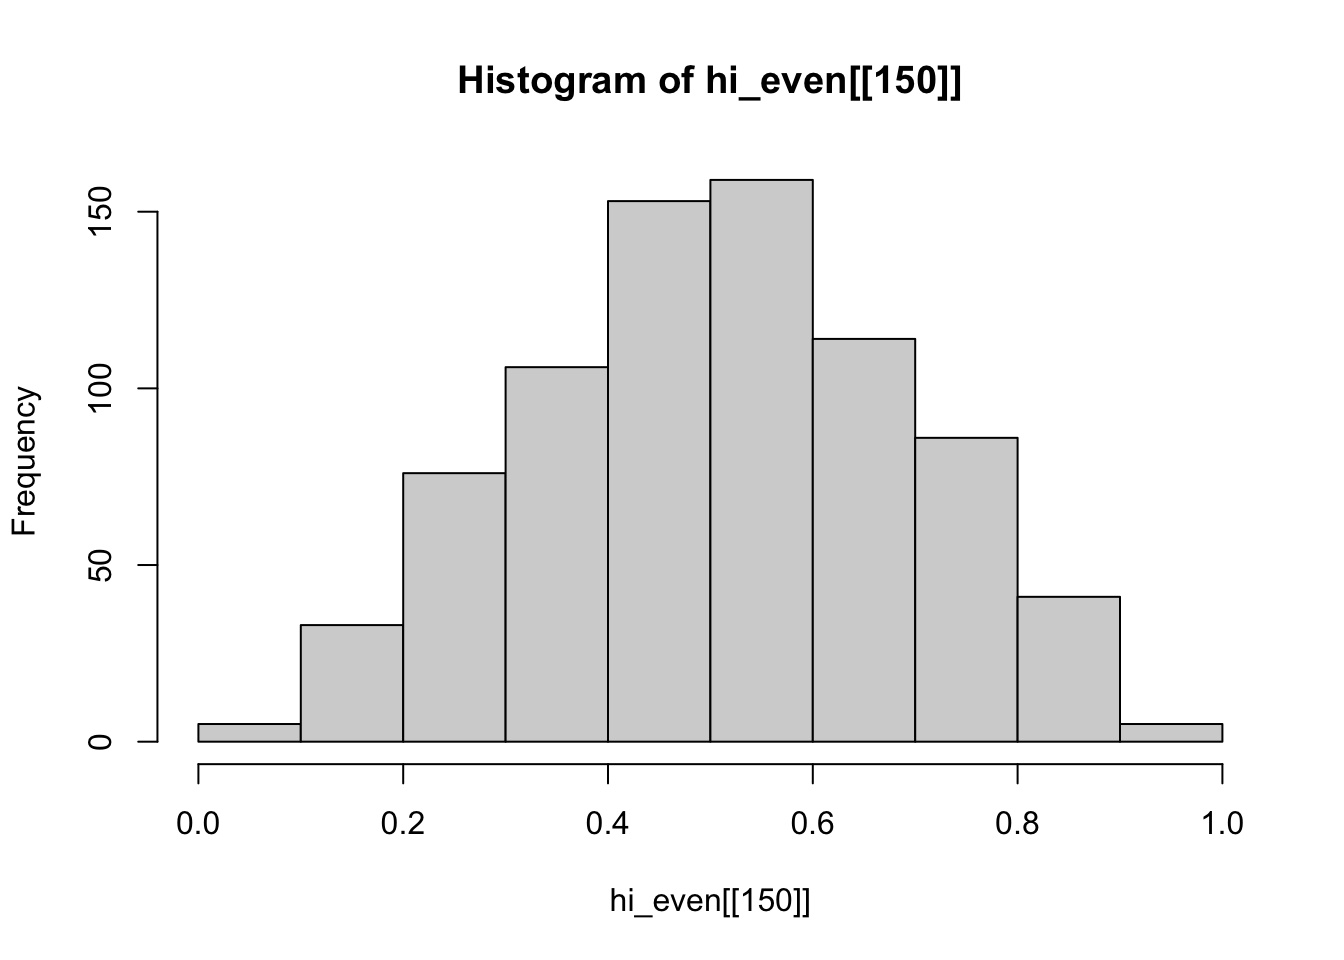
\includegraphics{gde_behavior_exploration_files/figure-latex/unnamed-chunk-9-1.pdf}
sorted bar plot. Notice how it is less dramatic of a decrease compared
to a community with less even genetic diversities.

\begin{Shaded}
\begin{Highlighting}[]
\FunctionTok{barplot}\NormalTok{(}\FunctionTok{sort}\NormalTok{(hi\_even[[}\DecValTok{150}\NormalTok{]], }\AttributeTok{decreasing =} \ConstantTok{TRUE}\NormalTok{))}
\end{Highlighting}
\end{Shaded}

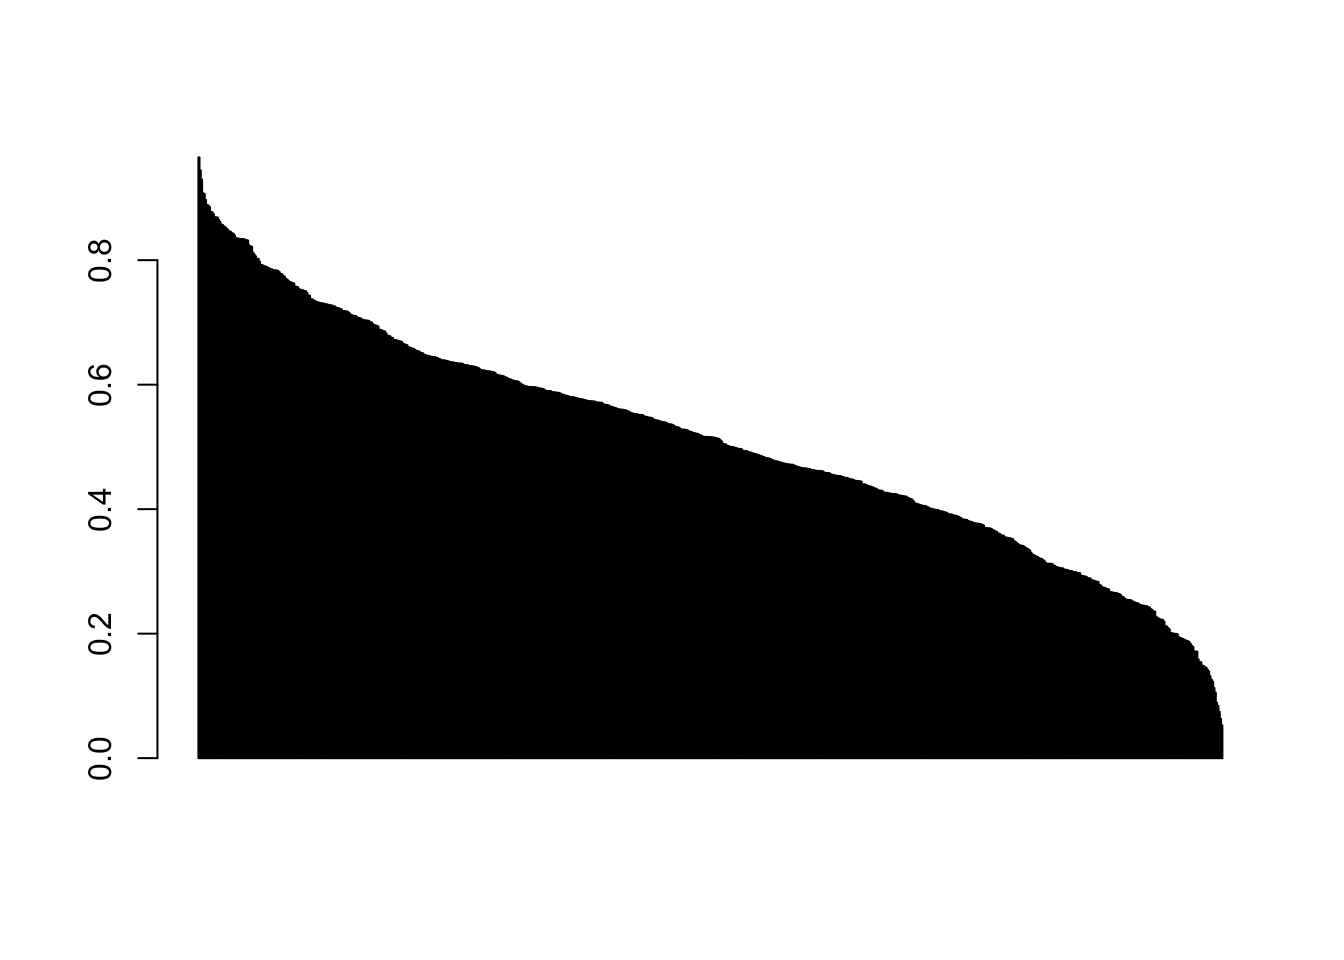
\includegraphics{gde_behavior_exploration_files/figure-latex/unnamed-chunk-10-1.pdf}

\begin{Shaded}
\begin{Highlighting}[]
\CommentTok{\# hill numbers are concentrated \textasciitilde{}0.925}
\FunctionTok{hist}\NormalTok{(}\FunctionTok{unlist}\NormalTok{(hi\_even\_hill))}
\end{Highlighting}
\end{Shaded}

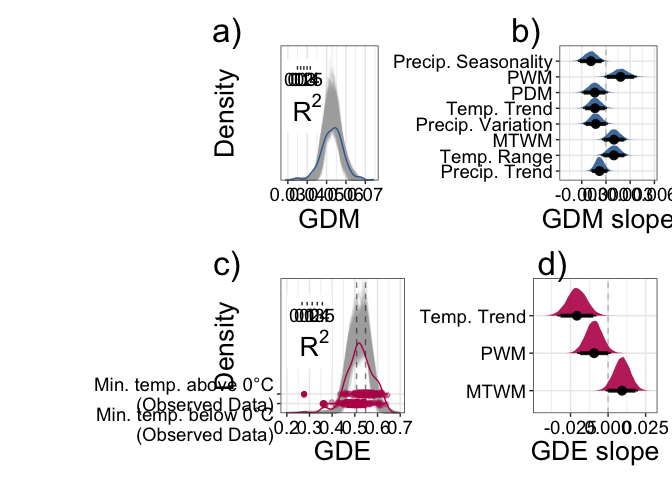
\includegraphics{gde_behavior_exploration_files/figure-latex/unnamed-chunk-11-1.pdf}

\begin{Shaded}
\begin{Highlighting}[]
\CommentTok{\# since the sample size vector is sorted, higher indices are higher sample sizes}
\CommentTok{\# looks like there is more variation at lower sample sizes}
\FunctionTok{plot}\NormalTok{(}\FunctionTok{unlist}\NormalTok{(hi\_even\_hill))}
\end{Highlighting}
\end{Shaded}

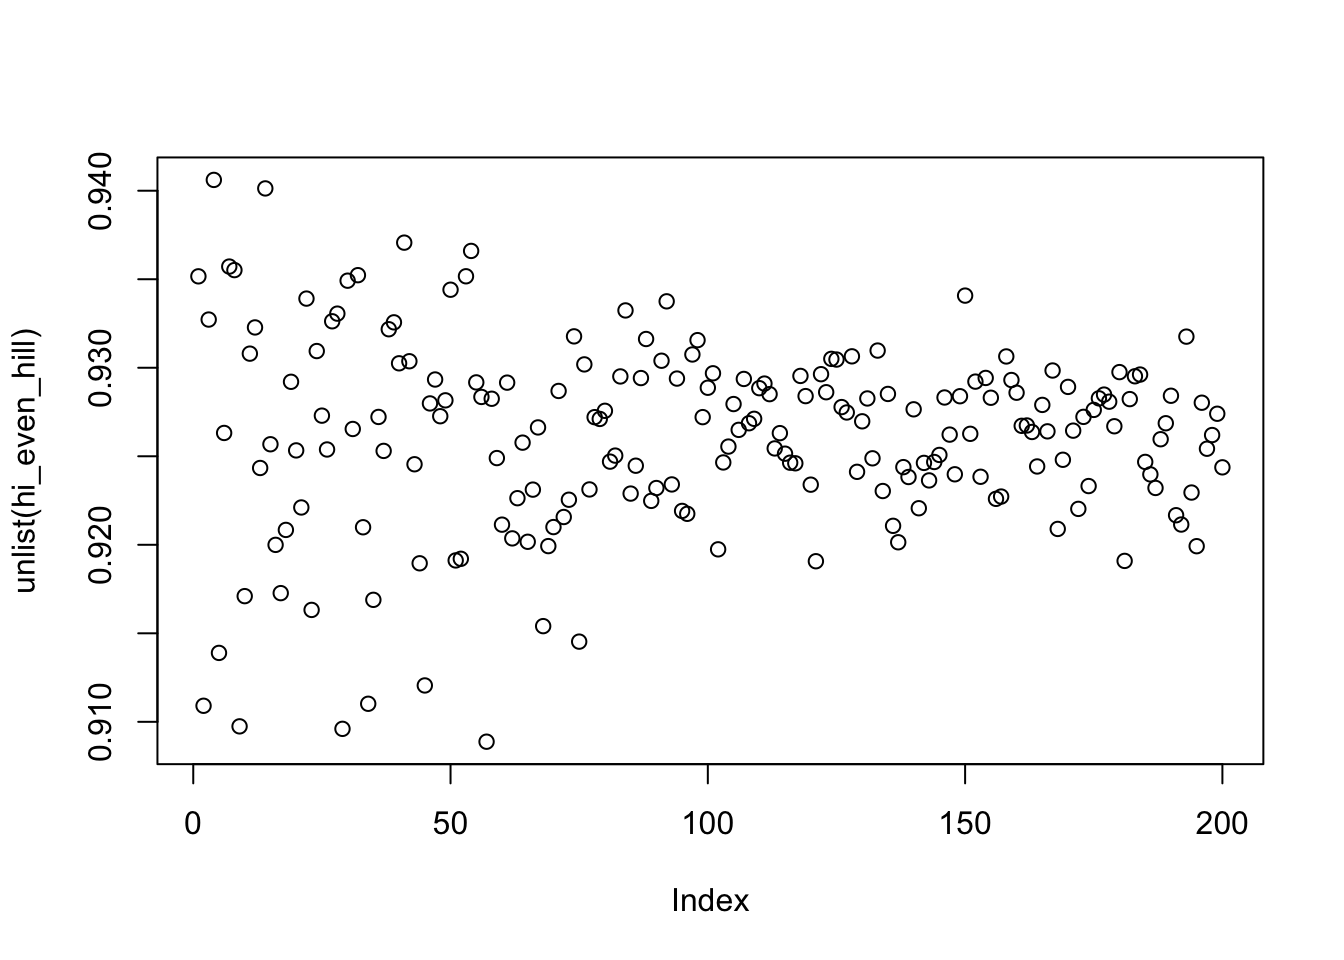
\includegraphics{gde_behavior_exploration_files/figure-latex/unnamed-chunk-12-1.pdf}

\end{document}
